\documentclass{llncs}
\usepackage[utf8]{inputenc}
\usepackage{fancyvrb} 
\usepackage[portuguese]{babel}
\usepackage{ragged2e}
\usepackage{graphicx}
\usepackage{float}

\begin{document} \mainmatter
\title{Processador de Thesaurus}
\titlerunning{Processador de Thesaurus}
\author{José Carlos Lima Martins A78821 \and
        Miguel Miranda Quaresma A77049}
\authorrunning{José Carlos Lima Martins A78821 \and
        Miguel Miranda Quaresma A77049}
\institute{                                                                
University of Minho, Department of  Informatics, Braga, Portugal\\
e-mail: \{a78821,a77049\}@alunos.uminho.pt
}

\maketitle

\justify

\begin{abstract}
Este documento serve de apoio ao desenvolvimento de um Processador Thesaurus explicando todas as decisões tomadas de modo a obter o mesmo. Inicialmente será explicitada a estrutura dos ficheiros de entrada (extensão .mdic) e identficadas as decisões tomadas de modo a obter a versão atual do processador. Em cada uma das fases do desenvolvimento serão apresentados exemplos de utilização do processador.
\end{abstract}

\section{Introdução}
O presente projeto (Processador de Thesaurus) visa ser um sistema de processamento de dicionários Thesaurus que recorre a expressões regulares (ERs) para filtrar e transformar os mesmos, extraindo e tratando a informação mais relevante de forma eficiente. Para atingir este objetivo é usada a linguagem de filtragem e tratamento de dados \texttt{AWK} visto ser uma \textbf{DSL}(Domain Specific Language) com foco em dados semi-estruturados.

\section{Preliminares}
De modo a compreender melhor o desenvolvimento deste projeto é importante compreender a estrutura dos dicionários Thesaurus(ficheiros .mdic). 
A estrutura de um dicionário pode ser dividido em três componentes principais:
\begin{itemize}
    \item linhas começadas por '\#': comentários a ignorar
    \item diretivas gerais:
        \begin{itemize}
            \item linhas começadas por '\%dom: dominio': indica que até ao aparecimento de nova linha começada por '\%dom:' todos os termos são de 'dominio', sendo dom uma relação e a sua inversa é voc
            \item linhas começadas por '\%inv: relação1 : relação2': indica que a relação1 tem como inversa a relação2
        \end{itemize}
    \item linhas começadas por '\%THE': indicam tabelas de relações, com as seguintes caracteristicas:
        \begin{itemize}
            \item a linha inicial possui as relações bem como as classes da coluna correspondente
            \item cada linha tem 1 ou mais termos, menos a inicial que possui apenas relações e classes
            \item os termos são separados por ':' daqueles com que se relacionam
            \item a relação entre o termo da coluna 1 e da coluna N é dado pela relação N da linha inicial
            \item na presença de vários termos com a mesma relação, podem ser agrupados por '$|$'
            \item quando uma relação na linha inicial possui $<$classe, ou seja 'relação$<$classe', significa que o elementos dessa coluna são instâncias da 'classe'
            \item quando '\%THE$<$classe' significa que o termo1 é instância da 'classe'
        \end{itemize}
\end{itemize}
Com esta estrutura em mente explicita-se, de seguida, o desenvolvimento do processado de Thesaurus.

\section{Desenvolvimento}
\subsection{Exe 1}
O processamento iniciou-se pela identificação dos domínios e relações presentes no dicionário. Para tal, e tendo em conta a estrutura dos documentos, foi usado como \texttt{Field Separator} o carácter ':'.
Tendo em conta a sintaxe de Padrão $\to$ Ação inerente ao \texttt{AWK} foram considerados relevantes os seguintes padrões:
\begin{enumerate}
    \item \verb|/^%dom/|: padrão que identifica novo domínio no início de uma linha
    \item \verb|/^%THE/|: padrão que identifica início de tabela de relações indicadas na presente linha
    \item \verb|/^%inv/|: padrão que identifica uma relação inversa à indicada no segundo campo
\end{enumerate}
No caso do padrão \verb|/^%dom/| a ação compreende a remoção de espaços que precedam o domínio e o armazenamento do mesmo numa matriz \texttt{ind}.
\begin{Verbatim}
    /^%dom/     {sub(/^ /,"",$2); ind[0][$2]++}
\end{Verbatim}
Quando o padrão encontrado é do tipo \verb|/^%THE/| ou \verb|/^%inv/| são percorridos todos os campos (\textbf{i.e.}relações) e quando uma dada relação não vazia (\verb|$j!=" " && $j!=""|) é encontrada são-lhe removidos os espaços precedentes e subsequentes removendo também, eventualmente, a indicação de classe. De seguida, estes são também armazenados na matriz \texttt{ind}.
\begin{Verbatim}
/^%(THE|inv)/   {for(j=2;j<=NF;j++){
                    if($j != " " && $j!=""){
                        sub(/^(\s)*/,"",$j);
                        sub(/(\s)|(<(.*)?)/,"",$j);
                        !ind[1][$j]++;
                    }
                }
                }
\end{Verbatim}

Por fim, quando o final de ficheiro é encontrado (\texttt{EOF}) são impressos os domínios e as relações recorrendo, para isso, às funções \texttt{printDominios} e \texttt{printRelations} respetivamente.

\subsubsection{Usage}
Dado a simplicidade do processador desenvolvido, um exemplo de uso consiste em identificar os domínios e relações presentes num dado dicionário *.mdic:
\begin{Verbatim}
    gawk -f exe1.awk *.mdic
\end{Verbatim}

\begin{figure}[H]
    \centering
    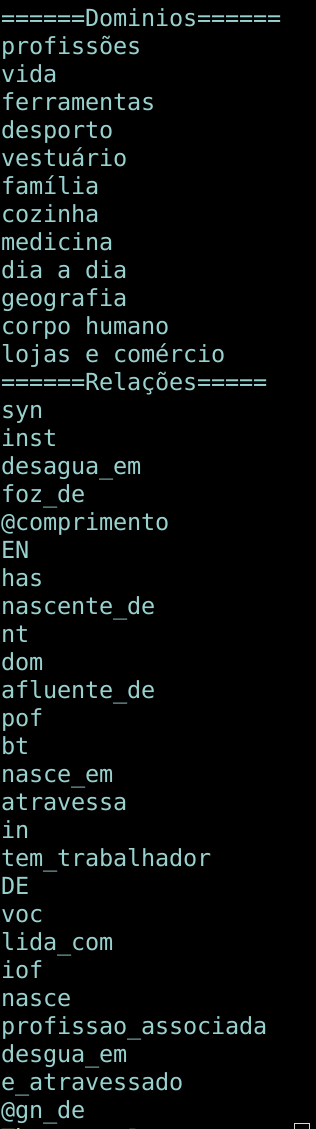
\includegraphics[height=7cm]{Exe1Out.png}
    \caption{Output de \texttt{gawk -f exe1.awk *.mdic}}
\end{figure}

\section{Exe 2}
O objetivo deste exercício é mostrar os triplos expandidos (um por cada linha) correspondentes às relações entre os termos. Como tal, é necessário percorrer os ficheiros por completo. Mais uma vez o carácter usado como \texttt{Field Separator} foi ':'. Consoante o início da linha, a ação levada a cabo é indicada de seguida:
\begin{itemize}
    \item \verb|/^%dom/|: guarda-se o dominio indicado numa variável até aparecer uma nova linha com o mesmo padrão altura em que o dominio é atualizado
    \item \verb|/^%inv/|: guarda num índice \texttt{inv} a relação e a sua respetiva inversa
    \item \verb|/^%THE/|: as relações são armazenadas num índice \texttt{relation} e as classes (quando aplicável/existentes) num índice \texttt{class}
    \item \verb|$1 !~/^%/ && $0 !~ /^#/ && $0 != ""| (\textbf{i.e.}tabelas de relações): os triplos são armazenados no índice \texttt{triples} da seguinte maneira e consoante as seguintes condições: 
        \begin{itemize}
            \item termo1 relacionado com o dominio(\textbf{dom}) bem como a respetiva inversa(\textbf{voc})
            \item caso exista uma classe associada ao '\%THE' é adicionado os triplos correspondentes ao \textbf{instance of}(iof) e \textbf{tem como instancia}(inst) envolvendo o termo1 e a classe
            \item são percorridos o resto dos campos (termos da lado direito), separando-os por $|$ usando o \texttt{split} obtendo os seguintes triplos dependendo do caso:
                \begin{itemize}
                    \item os triplos que relacionam o termo com o dominio (dom e voc)
                    \item o triplo envolvendo o termo1, a relação da coluna correspondente e o termo, sendo que caso a relação possua inversa(verificado no indice inv) é adicionado o triplo
                    \item caso a coluna possua classe, o termo é relacionado com a mesma(iof e inst)
                \end{itemize}
        \end{itemize}
\end{itemize}
Após o armazenamento de todos os triplos no índice \texttt{triples}, ou seja após percorridos todos os ficheiros(\textbf{END}) é percorrido esse mesmo índice imprimindo cada triplo. Este índice usa o triplo como método de indexação e, em cada posição, guarda um inteiro que indica a ocorrência(1)  ou não(0) do triplo, permitindo assim impedir a duplicação de informação. É importante referir que todos os elementos, sejam classes, relações ou termos, são tratados de modo a lhes serem retirado espaços que estejam antes e após os mesmos.

\subsubsection{Usage}
O exemplo mais comum de utilização deste programa é:
\begin{verbatim}
gawk -f exe2.awk *.mdic
\end{verbatim}
Pode ser também interessante guardar o resultado num ficheiro:
\begin{verbatim}
gawk -f exe2.awk *.mdic >> file.txt
\end{verbatim}

\begin{figure}[H]
    \centering
    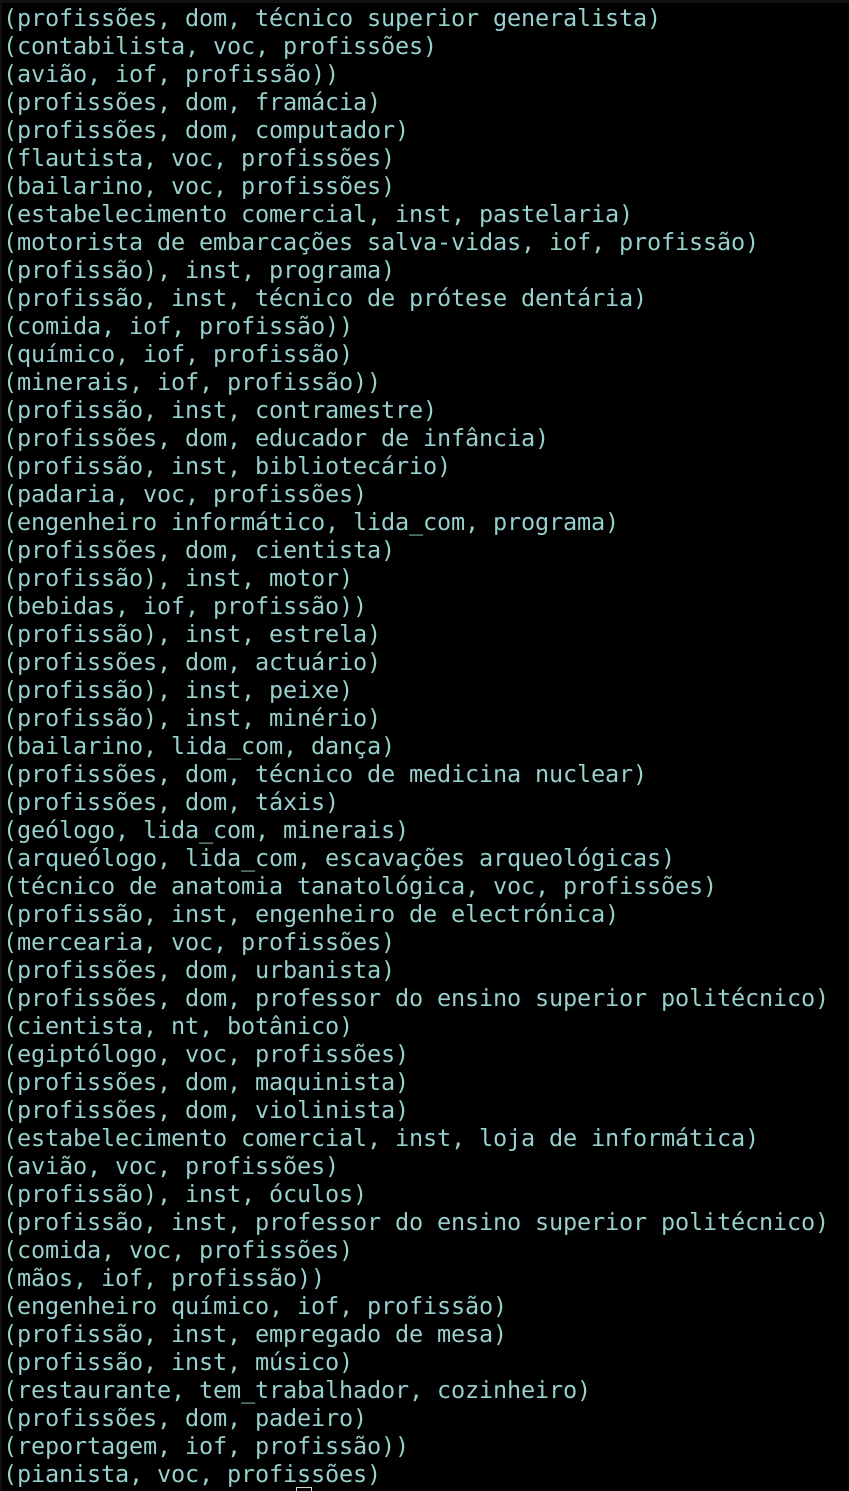
\includegraphics[height=7cm]{Exe2Out.png}
    \caption{Sample output de \texttt{gawk -f exe2.awk profissoes-lojas.mdic}}
\end{figure}

\subsection{Exe 3}
O último exercício compreende a criação de ficheiros \texttt{HTML} com hiperligações entre si com base nos termos e nas suas relações \textbf{i.e.} nos triplos construídos no exemplo anterior. Para obter este resultado basta recorrer ao código desenvolvido no exercício anterior e, quando o fim do ficheiro for encontrado, criar as hiperligações referidas. 
Como tal, neste exercício é usado como \textit{input} o \textit{output} do exercício anterior e, para cada triplo, são removidos os parêntesis, dividindo de seguida os termos pelas vírgulas, e removendo a cada termo os espaços precedentes e subsequentes. Os termos são guardados num índice \textit{triples}, separados por uma virgula (\verb|triples[i]=triple[1] "," triple[3];|). Cada \textbf{termo1} é armanzenado num índice \texttt{ind} de modo a registar todos os ficheiros \texttt{HTML} (e correspondentes hiperligações) que serão criados. No fim do ficheiro(\textbf{END}), é percorrida a lista de triples e, para cada novo elemento é criado o ficheiro \texttt{HTML} correspondente com a tag de \textit{enconding} e de lista:

\begin{verbatim}
if(create[aux[1]]==""){
    print "<meta charset=\"utf-8\">" >> aux[1] ".html";
    print "<ul>" >> aux[1] ".html";
    !create[aux[1]]++;
}
\end{verbatim}

A criação de hiperligações é precedida de uma verificação em relação à existência do ficheiro a que esta se refere e, caso este não exista, é apenas criado um item com o nome do \textbf{termo2} correspondente.

\begin{verbatim}
if(ind[aux[2]]!="") 
    print "<li><a href=\"" aux[2] ".html\">" aux[2] "</a></li>" >> aux[1] ".html"
else print "<li>" aux[2] "</li>" >> aux[1] ".html"
\end{verbatim}

Após todas as hiperligações terem sido criadas é adicionada a macro de fecho de lista (\textbf{$<$/ul$>$})a todos os ficheiros criados , recorrendo para isso ao índice \texttt{create}:
\begin{verbatim}
for(y in create){
    print "</ul>" >> y ".html";
}
\end{verbatim}

\subsubsection{Usage}
Como anteriormente referido foi usado o \textit{output} do exercicio anterior e, de modo a obter os resultados esperados, o programa deve ser executado, preferencialmente, de uma das seguintes maneiras:
\begin{itemize}
    \item \begin{verbatim}
    gawk -f exe2.awk *.mdic | gawk -f exe3.awk
    \end{verbatim}
    \item \begin{verbatim}
    gawk -f exe2.awk *.mdic >> file.txt
    gawk -f exe3.awk file.txt
    \end{verbatim}
\end{itemize}

\begin{figure}[H]
    \centering
    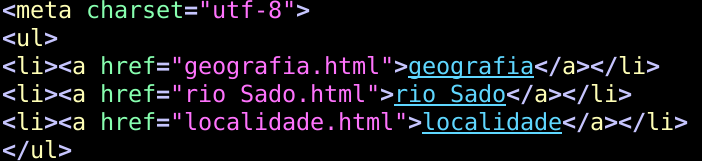
\includegraphics[height=3cm]{Exe3Out.png}
    \caption{Ficheiro "Alcácer do Sal.html"  resultante de \texttt{gawk -f exe2.awk riospt.mdic >> file.txt \&\& cat file.txt $|$ gawk -f exe3.awk}}
\end{figure}

\section{Conclusão}
O uso de uma linguagem \textbf{DSL} de \textit{scripting} como o \texttt{AWK} permite o rápido desenvolvimento de um processador de dados semi-estruturados nomeadamente um dicionário Thesaurus. Este tipo de processador necessitaria de código de complexidade superior e de tamanho considerável caso fosse desenvolvido em linguagens declarativas como C ou Java em que é necessário ter em conta a gestão da memória bem como outras trivialidades que são de pouca relevância para o processador em si. Em \texttt{AWK}, dada a sua estrutura \textbf{padrão $\to$ ação}, o código desenvolvido é conciso e de fácil leitura.

\end{document}
